\begin{abstractbook}
\textbf{\begin{center}\end{center}}
Caution : You need to give an English Abstract by begin-abstractbook.This is a template for SJTU speech lab tech reports.
\end{abstractbook}

\section{Task}
\label{sec:intro}
%\usepackage{indentfirst}
%\setlength{\parindent}{2em} 
The Task for Assignment 1 is it to evaluate a histogram equalizer. The methods of implementing this histogram equalizer are not specified which means that every student can use different approaches.

\section{Implementation}

My implementation was done using python, especially numpy and scipy. Generally the implementation follows three steps:

\begin{enumerate}
\item For the ith element in k-graylevels , we firstly estimate the counts by using the current pixel $p(x,y)$ \begin{equation}
c_i = \sum\limits_{i=0}^{k-1} p(x,y) = i
\end{equation}

\item Afterwards the distribution is calculated by using \begin{align}
\frac{c_i}{c} \\
c = \sum\limits_i c_i
\end{align}

\item The cdf is then calculated by summing up the last j frames of i. Furthermore these cdf's need to evaluated by multiplying them by the Grayscale-1, to find an appropriate mapping into the new space.
\begin{align}
cdf_i = \sum\limits_{b=0}^{j=i} c_b \\
new_i = cdf_i * 255
\end{align}

\item Finally the old pixels need to be mapped into the new space, where a simple lookup in the $new_i$ array is sufficient.

\end{enumerate}


\section{Usage}

The written program can be used with the following syntax.

\begin{lstlisting}
python __init__.py inputimagepath -oh1 orighistpath -oh2 transhistpath -o pictureoutpath
\end{lstlisting}

The results can be seen below

\begin{figure}[htbp]
\centering
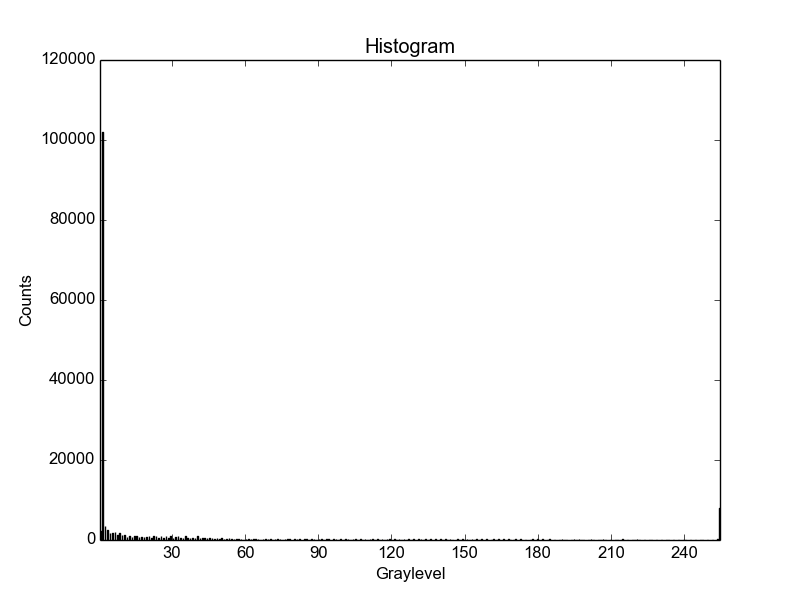
\includegraphics[width=14cm]{histoOrigFig1.png}
\caption{Original Histogram of Figure 1}
\label{fig:abc}
\end{figure}
\begin{figure}[htbp]
\centering
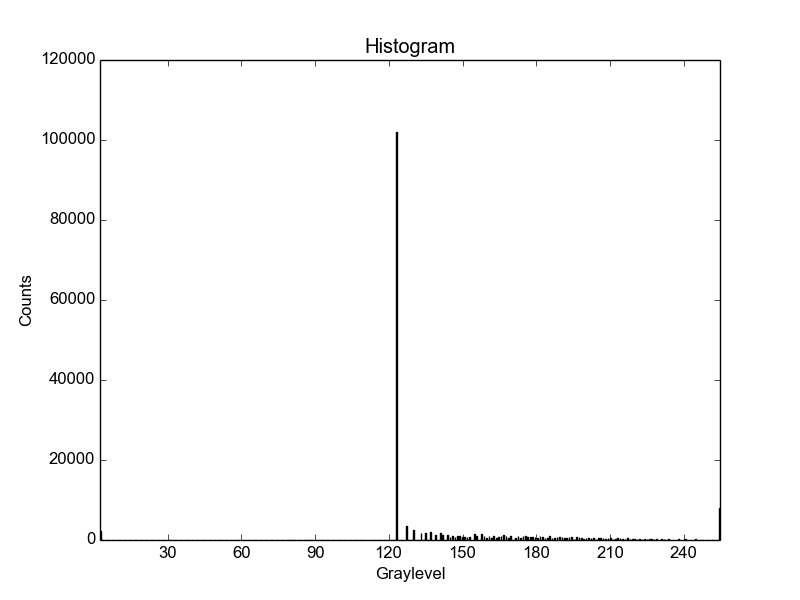
\includegraphics[width=14cm]{histoTransFig1.png}
\caption{Transformed Histogram of Figure 1}
\label{fig:abc}
\end{figure}
\begin{figure}[htbp]
\centering
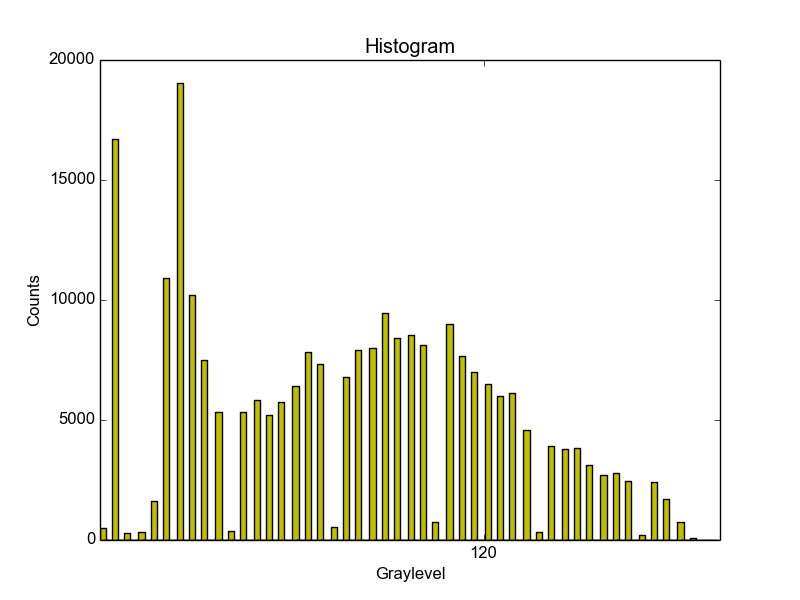
\includegraphics[width=14cm]{histoOrigFig2.png}
\caption{Original Histogram of Figure 2}
\label{fig:abc}
\end{figure}
\begin{figure}[htbp]
\centering
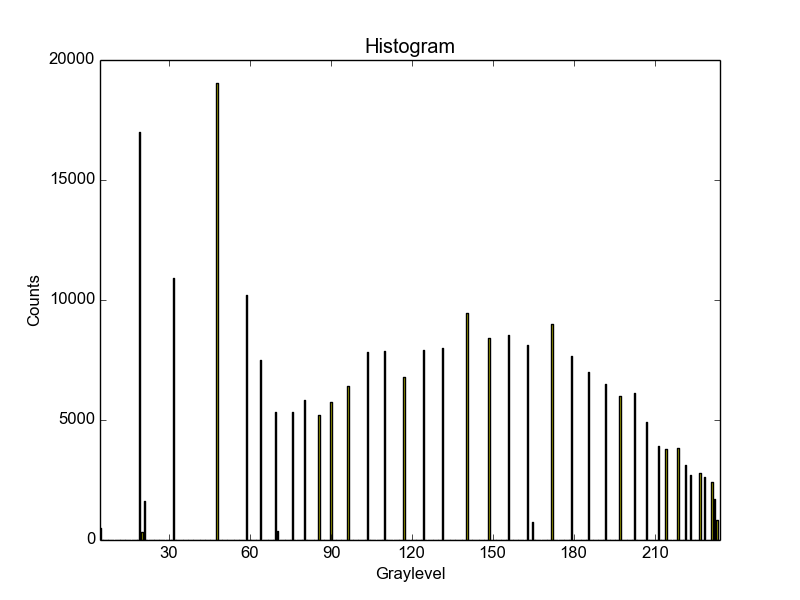
\includegraphics[width=14cm]{histoTransFig2.png}
\caption{Transformed Histogram of Figure 2}
\label{fig:abc}
\end{figure}
\begin{figure}[htbp]
\centering
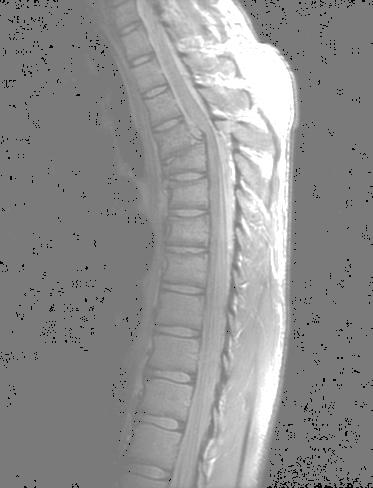
\includegraphics[width=14cm]{fig1out.jpg}
\caption{Output image of Figure 1}
\label{fig:abc}
\end{figure}
\begin{figure}[htbp]
\centering
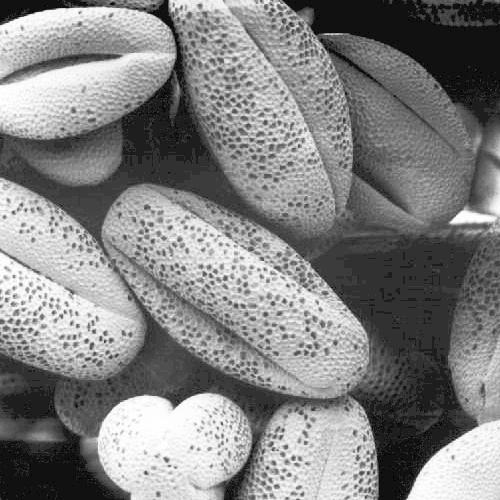
\includegraphics[width=14cm]{fig2out.jpg}
\caption{Output image of Figure 2}
\label{fig:abc}
\end{figure}
